

%%%%%%%%%%%%%%%%%%%%%%%%%%%%%%%%%%%%%%%%%
% University/School Laboratory Report
% LaTeX Template
% Version 3.1 (25/3/14)
%
% This template has been downloaded from:
% http://www.LaTeXTemplates.com
%
% Original author:
% Linux and Unix Users Group at Virginia Tech Wiki 
% (https://vtluug.org/wiki/Example_LaTeX_chem_lab_report)
%
% License:
% CC BY-NC-SA 3.0 (http://creativecommons.org/licenses/by-nc-sa/3.0/)
%
%%%%%%%%%%%%%%%%%%%%%%%%%%%%%%%%%%%%%%%%%

%----------------------------------------------------------------------------------------
%	PACKAGES AND DOCUMENT CONFIGURATIONS
%----------------------------------------------------------------------------------------

\documentclass{article}

\usepackage[version=3]{mhchem} % Package for chemical equation typesetting
\usepackage{siunitx} % Provides the \SI{}{} and \si{} command for typesetting SI units
\usepackage{graphicx} % Required for the inclusion of images
\usepackage{natbib} % Required to change bibliography style to APA
\usepackage{amsmath} % Required for some math elements 
\usepackage{listings}
\usepackage{color}
\usepackage{caption}
\usepackage{rotating}
\usepackage{enumitem}
\usepackage{url}
%\usepackage{hyperref}

\definecolor{dkgreen}{rgb}{0,0.6,0}
\definecolor{gray}{rgb}{0.5,0.5,0.5}
\definecolor{mauve}{rgb}{0.58,0,0.82}

\lstset{frame=tb,
  language=Java,
  aboveskip=3mm,
  belowskip=3mm,
  showstringspaces=false,
  columns=flexible,
  basicstyle={\small\ttfamily},
  numbers=none,
  numberstyle=\tiny\color{gray},
  keywordstyle=\color{blue},
  commentstyle=\color{dkgreen},
  stringstyle=\color{mauve},
  breaklines=true,
  breakatwhitespace=true,
  tabsize=3
}
\setlength\parindent{0pt} % Removes all indentation from paragraphs

\renewcommand{\labelenumi}{\alph{enumi}.} % Make numbering in the enumerate environment by letter rather than number (e.g. section 6)

%\usepackage{times} % Uncomment to use the Times New Roman font

%----------------------------------------------------s------------------------------------
%	DOCUMENT INFORMATION
%----------------------------------------------------------------------------------------

\title{Laboratory Assignment 7 Write Up \\ Computer Science 441} % Title

\author{\textsc{Andreas Bach Landgrebe}} % Author name

\date{\today} % Date for the report

\begin{document}

\maketitle % Insert the title, author and date

\begin{center}
\begin{tabular}{l r}
Date Submitted:  March 14, 2016 \\ % Date the experiment was performed
Partners:  Andreas Bach Landgrebe  \\ % Partner names
Instructor:  Dr. Gregory M. Kapfhammer  % Instructor/supervisor
\end{tabular}
\end{center}

% If you wish to include an abstract, uncomment the lines below
% \begin{abstract}
% Abstract text
% \end{abstract}

%----------------------------------------------------------------------------------------
%	SECTION 1
%----------------------------------------------------------------------------------------

\section{The well-commented source code of all of the Java classes in the final distributed system.}
\textbf{Simple.java}
\begin{lstlisting}
import java.io.File;
import java.io.IOException;
import java.io.InputStream;
import java.io.OutputStream;
import java.rmi.RemoteException;

/**
 * @author pothoven
 *
 */
/**
 * @author pothoven
 *
 */
public interface Simple extends java.rmi.Remote {
  /**
   * check if server is available
   *
   * @return
   * @throws RemoteException
   */
  String ping() throws RemoteException;
  //ping method being used to send a simple hello world message from the client to the server
  /**
   * run a command on the report server
   *
   * @param command
   * @param envp
   * @return
   * @throws RemoteException
   */
  String runCommand(String command, String[] envp) throws RemoteException;
  //method being used to run a command


  /**
   * Get an output stream for a file to allow file downloads
   *
   * @param File f
   * @return
   * @throws IOException
   */
  OutputStream getOutputStream(File f) throws IOException;
  //method being used to get an output stream

  /**
   * Get an input stream for a file to allow file uploads
   *
   * @param File f
   * @return
   * @throws IOException
   */
  InputStream getInputStream(File f) throws IOException;
  //method being used to get the input stream
}

\end{lstlisting}

\textbf{SimpleClient.java}

\begin{lstlisting}
import java.io.File;
import java.io.FileInputStream;
import java.io.FileOutputStream;
import java.io.IOException;
import java.io.InputStream;
import java.io.OutputStream;
import java.rmi.Naming;
import java.rmi.registry.Registry;
import java.util.MissingResourceException;
import java.util.PropertyResourceBundle;
import java.util.ResourceBundle;

public class SimpleClient
{
  final public static int BUF_SIZE = 1024 * 64;

  /**
   * Copy the input stream to the output stream
   *
   * @param in
   * @param out
   * @throws IOException
   */
  public static void copy(InputStream in, OutputStream out)
    throws IOException {

    byte[] b = new byte[BUF_SIZE];
    int len;
    while ((len = in.read(b)) >= 0) {
      out.write(b, 0, len);
    }
    in.close();
    out.close();
  }

  public static void upload(Simple server, File src, File dest) throws IOException {
    copy (new FileInputStream(src), server.getOutputStream(dest));
    //upload a file between the client and the server. 
  }

  public static void download(Simple server, File src, File dest) throws IOException {
    copy (server.getInputStream(src), new FileOutputStream(dest));
    //download a file between the client and the server.
  }

  public static void main(String arg[])
  {
    //main method
    ResourceBundle properties = PropertyResourceBundle.getBundle("Simple");
    int port = Registry.REGISTRY_PORT;
    //int data port used for to store the port
    try {
      port = Integer.parseInt(properties.getString("server.port"));
      //parse the int to a string for the server port
    } catch (Exception e) {
      port = Registry.REGISTRY_PORT;
    }
    String command = null;
    if (arg.length > 0) {
      //if the length of the argument is greater than 0, then start the String at the first index of the array. 
      command = arg[0];
    }

    if (command != null && command.length() > 0) {

      boolean useSecurityManager = false;
      //if statement for security manager if addes security was used between the client and the server. 
      try {
        Boolean.valueOf(properties.getString("useSecurityManager"));
      } catch (Exception e) {
        // default to false
      }
      if (useSecurityManager && System.getSecurityManager() == null) {
        System.setSecurityManager(new SecurityManager());
      }

      try
      //catch the connection between the client and the server. The server.ip would be the localhost.
      {
        String serverIP = System.getProperty("server.ip");
        if (null == serverIP) {
          try {
            serverIP = properties.getString("server.ip");
          } catch (MissingResourceException e) {
            //catch the exception if it is not working properly. 
            throw new Exception("Undefined server IP.  Please define 'server.ip' as system property (ex. java -Dserver.ip=xxx) or in the Simple.properties file.");
          }
        }

        Simple server = (Simple) Naming.lookup( "//" +
            serverIP +
            ":" + port +
            "/SimpleServer");

        if ( command.equalsIgnoreCase("ping") ) {
          //if ping is being called as an argument, then run the ping method.
          //the ping method will send the "Hello, world!" message to the server from the client
          System.out.println(server.ping());

        } else if (command.equalsIgnoreCase("upload") ) {
          //if upload is being called as an argument, then run the upload method
          //the upload method will specify a local file to be uploaded
          //if the length of the argument is more than one, then the second argument is the remote file to be written to. 
          if (arg.length > 1) {
            String srcFilename = arg[1];
            if (srcFilename != null && srcFilename.length() > 0) {
              String destFilename = srcFilename;
              if (arg.length > 2) {
                destFilename = arg[2];
              }
              upload(server, new File(srcFilename), new File(destFilename));
            }
          }

        } else if (command.equalsIgnoreCase("download") ) {
          //if download is being called as an argument, then run the download method
          //the download method will specify a remote file to be downloaded
          //if the length of the argument is more than one, then the second argument is the local file to be written to.
          if (arg.length > 1) {
            String srcFilename = arg[1];
            if (srcFilename != null && srcFilename.length() > 0) {
              String destFilename = srcFilename;
              if (arg.length > 2) {
                destFilename = arg[2];
              }
              download(server, new File(srcFilename), new File(destFilename));
            }
          }

        } else {
          System.out.println(server.runCommand(command, null));
        }
      }
      catch (Exception e)
      {
        //catch the exception
        System.out.println("SimpleClient exception: " + e.getMessage());
        e.printStackTrace();
      }
    } else {
      //print the commands if they are not being used correctly.
      System.out.println("Usage: SimpleClient command");
      System.out.println("\nExample: java [-Djava.security.policy=rmi.policy] -jar simple-client.jar ping");
      System.out.println("\n         java [-Djava.security.policy=rmi.policy] -jar simple-client.jar upload srcfile.txt [destfile.txt]");
      System.out.println("\n         java [-Djava.security.policy=rmi.policy] -jar simple-client.jar download afile.txt [destfile.txt]");
      System.out.println("\n         java [-Djava.security.policy=rmi.policy] -jar simple-client.jar \"db2 reorg indexes all for table ADWSRNCT.F_INCIDENT\"");
    }
  }
}

\end{lstlisting}

\textbf{SimpleServer.java}

\begin{lstlisting}
//import statements
import java.rmi.registry.LocateRegistry;
import java.rmi.registry.Registry;
import java.util.PropertyResourceBundle;
import java.util.ResourceBundle;

/**
 * @author pothoven
 *
 */
public class SimpleServer
{

  public static void main(String args[])
  {
    ResourceBundle properties = PropertyResourceBundle.getBundle("Simple");
    //ResourceBundle object to get an object from the client
    int port = Registry.REGISTRY_PORT;
    //integer used for the port
    try {
      port = Integer.parseInt(properties.getString("server.port"));
      //try the connection on this server port
    } catch (Exception e) {
      // default to Registry.REGISTRY_PORT
    }

    try
    {
      boolean useSecurityManager = false;
      //set the security protocol to be false
      try {
        Boolean.valueOf(properties.getString("useSecurityManager"));
        //try to use the security manager if the above boolean was changed to true.
      } catch (Exception e) {
        // default to false
      }

      if (useSecurityManager && System.getSecurityManager() == null) {
        //this is all used for the security manager if you specify it in the command line.
        System.setSecurityManager(new SecurityManager());
        //setting the securtity up if it is being used.
      }

      Registry registry = LocateRegistry.createRegistry(port);
      //registry object with the port specified.

      SimpleImpl obj = new SimpleImpl();
      /* Bind this object instance to the name "SimpleServer" */
      // Naming.rebind("SimpleServer", obj);
      registry.rebind("SimpleServer", obj);

      System.out.println("SimpleServer started on port " + port);
        //started up the server and specifiy the port that it started on
    }
    catch (Exception e)
    //if the server is not able to start, catch the exception
    {
      System.out.println("SimpleServer err: " + e.getMessage());
      e.printStackTrace();
    }
  }
}

\end{lstlisting}

\textbf{SimpleImpl.java}

\begin{lstlisting}
import io.RMIInputStream;
import io.RMIInputStreamImpl;
import io.RMIOutputStream;
import io.RMIOutputStreamImpl;

import java.io.BufferedReader;
import java.io.File;
import java.io.FileInputStream;
import java.io.FileOutputStream;
import java.io.IOException;
import java.io.InputStream;
import java.io.InputStreamReader;
import java.io.OutputStream;
import java.rmi.RemoteException;
import java.rmi.server.UnicastRemoteObject;
import java.util.Vector;

/**
 * @author pothoven
 *
 */
public class SimpleImpl extends UnicastRemoteObject implements Simple {
  /**
   *
   */
  private static final long serialVersionUID = 1L;

  public static final int DEFAULT_MAX_THREAD_COUNT = 5;

  private static Vector<Thread> pendingCommandThreads = new Vector<Thread>();
  //pending the running the command threads using a vector.
  private static Vector<Thread> runningCommandThreads = new Vector<Thread>();

  public SimpleImpl() throws RemoteException {}

  /* (non-Javadoc)
   * @see Simple#ping()
   */
  @Override
  public String ping() { return "Hello world!"; }
  //if you speicify ping in the command line, the client will send the server the message "Hello world!"


  /* (non-Javadoc)
   * @see Simple#runCommand(java.lang.String, java.lang.String[])
   */
  @Override
  public String runCommand(String command, String[] envp)
  throws RemoteException {
    //running the command

  CommandThread t = new CommandThread(command, envp);
  //command thread object
  try {

    if (getActiveThreadCount() < getMaxThreadCount()) {
      //if the active thread count is less than max thread count, then the whole vector<thread> has not been processed
      runningCommandThreads.add(t); //adding the common thread to the end of the vector 
      t.start(); //starting the common thread
      //
    } else {
      pendingCommandThreads.add(t); //adding the common thread to the end of the vector
      System.out.println("Queued (thread: " + t.getName() + "): " + command); //print debugging information to ensure the command is running correctly.
    }
    t.join(); //waits for this common thread to die

  } catch (Exception e) { //catch the exception if it does not work correctly.
    throw new RemoteException(e.getMessage());
  }

  return t.getResults(); //return the results.
  }

  /* (non-Javadoc)
   * @see Simple#getOutputStream(java.io.File)
   */
  public OutputStream getOutputStream(File f) throws IOException {
    //get the output stream
    System.out.println("Upload file: " + f.getName());
    //print the name of the upoload file between the client and the server
    return new RMIOutputStream(new RMIOutputStreamImpl(new FileOutputStream(f)));
    //return the output stream
  }

  /* (non-Javadoc)
   * @see Simple#getInputStream(java.io.File)
   */
  public InputStream getInputStream(File f) throws IOException {
    //get the input stream
    System.out.println("Download file: " + f.getName());
    //print the name of the downloaded file
    return new RMIInputStream(new RMIInputStreamImpl(new FileInputStream(f)));
    //return the input stream
  }

  /**
   * Get the number of pending command threads.
   *
   * @return number of pending command threads
   */
  public static int getPendingThreadCount() {
    //get the pending thread count method
    return pendingCommandThreads.size();
    //return the size of the thread
  }

  /**
   * Get the number of active command threads.
   *
   * @return number of active command threads
   */
  public static int getActiveThreadCount() {
    //get the active thread count
    return runningCommandThreads.size();
    //return the size of the thread count
  }

  protected int  getMaxThreadCount() { return DEFAULT_MAX_THREAD_COUNT; }
  //return the maximum thread count

  class CommandThread extends Thread {
    private String command = null; //string data type to store the command being used in the command line
    private String[] envp = null; //string array data type.
    private StringBuffer results = new StringBuffer(); // data type being used for the results

    public CommandThread(String command, String[] envp) {
      //constructor
      super(); //calls the parent constructor with no arguments
      this.command = command; //
      this.envp = envp;
    }

    public void run() {
      long startTime = System.currentTimeMillis();
      //start the timing between the client and the server

      // give a random time up to 2 sec delay before starting new threads
      // (if this isn't the first thread) to help prevent traffic jams
      if (SimpleImpl.getActiveThreadCount() > 1)
      {
        try {
          sleep((long) (Math.random() * 2000));
          //causes the currently executing thread to sleep for the specified number of milliseconds. 
        } catch (InterruptedException e1) { }
      }

      try {
        System.out.println("Running (thread: " + this.getName() + ") : " + command);
        //print the name of the thread with the command

        Process cmdProcess = Runtime.getRuntime().exec(command, envp);
        //command process 

        BufferedReader stdInput = new BufferedReader(new
            InputStreamReader(cmdProcess.getInputStream()));
        //get the input stream

        BufferedReader stdError = new BufferedReader(new
            InputStreamReader(cmdProcess.getErrorStream()));
        //get the error stream  
        String s = null;

        /* read the output from the command */
        while ((s = stdInput.readLine()) != null) {
          results.append(s);
        }

        /* read any errors from the attempted command  */
        while ((s = stdError.readLine()) != null) {
          results.append(s);
        }

      } catch (IOException e) {
        results.append(e.getMessage());
      } finally {
        long endTime = System.currentTimeMillis();
        //end the timing between the client and the server
        runningCommandThreads.remove(this);
        //print the thread when it is completed
        System.out.println("Completed (thread: " + this.getName() + ") in "+(endTime - startTime) + " ms");

        // start up the next pending thread
        if (getPendingThreadCount() > 0 &&
            getActiveThreadCount() < getMaxThreadCount()) {
          //if the thread count is still not the end of the file, then keep going.
          Thread t = pendingCommandThreads.remove(0);
        //add to the thread
          runningCommandThreads.add(t);
          t.start();
          //starting the common thread
            }
      }
    }

    /**
     * @return the results
     */
    public String getResults() {
      return results.toString();
      //return the results in a toString() method
    }

  }
}

\end{lstlisting}

\textbf{RMIInputStream.java}

\begin{lstlisting}
package io;

import java.io.IOException;
import java.io.InputStream;
import java.io.Serializable;

/**
 * from https://www.censhare.com/en/insight/overview/article/file-streaming-using-java-rmi
 */

/**
 * @author pothoven
 *
 */
public class RMIInputStream extends InputStream implements Serializable {

    /**
	 * 
	 */
	private static final long serialVersionUID = 1L;
	
	RMIInputStreamInterf in;
    
    public RMIInputStream(RMIInputStreamInterf in) {
        this.in = in;
        //inputn steam method
    }
    
    public int read() throws IOException {
        return in.read();
        //reading the input stream
    }

    public int read(byte[] b, int off, int len) throws IOException {
        //reading the input stream with different parameters
        byte[] b2 = in.readBytes(len);
        //reading the bytes
        if (b2 == null)
            //if b2 == 
            return -1;
        int i = b2.length; //set int i to the length of the bytes arrat being used. 
        System.arraycopy(b2, 0, b, off, i);
        //copy the bytes[] array
        return i;
    }
    
    public void close() throws IOException {
        super.close();
        //close the input stream
    }
}

\end{lstlisting}

\textbf{RMIInputStreamImpl}

\begin{lstlisting}
package io;

import java.io.IOException;
import java.io.InputStream;
import java.rmi.RemoteException;
import java.rmi.server.UnicastRemoteObject;

/**
 * from https://www.censhare.com/en/insight/overview/article/file-streaming-using-java-rmi
 */


/**
 * @author pothoven
 *
 */
public class RMIInputStreamImpl implements RMIInputStreamInterf {
	 private InputStream in;
	 //input stream object
	    private byte[] b;
	    //byte object

	    public RMIInputStreamImpl(InputStream in) throws IOException {
	        this.in = in;
	        UnicastRemoteObject.exportObject(this, 1099);
	        //export the object of the input stream specfying the port
	    }

	    public void close() throws IOException, RemoteException {
	        in.close();
	        //close the input stream
	    }

	    public int read() throws IOException, RemoteException {
	        return in.read();
	        //reading the input stream
	    }

	    public byte[] readBytes(int len) throws IOException, 
	            RemoteException {
	            	//method used to read the bytes
	        if (b == null || b.length != len)
	        	//if there is nothing in the bytes data types or it doesn't equal to int len parameter, then new bytes will be used
	            b = new byte[len];
	            //read the bytes in a new int primitve data type.
	        int len2 = in.read(b);
	        if (len2 < 0) //if len2 does not equal 0, then you have reached the end of the final.
	            return null; // EOF reached
	        
	        if (len2 != len) { //if the two int of len2 and len does not equal each other, then copy bytes to byte[] to correct length and return it.
	            // copy bytes to byte[] of correct length and return it
	            byte[] b2 = new byte[len2];
	            System.arraycopy(b, 0, b2, 0, len2);
	            return b2;
	        }
	        else
	            return b;
	    }
}

\end{lstlisting}

\textbf{RMIInputStreamInterf.java}

\begin{lstlisting}
package io;

import java.io.IOException;
import java.rmi.Remote;
import java.rmi.RemoteException;

/**
 * from https://www.censhare.com/en/insight/overview/article/file-streaming-using-java-rmi
 */

/**
 * @author pothoven
 *
 */
public interface RMIInputStreamInterf extends Remote {
    //input stream
    public byte[] readBytes(int len) throws IOException, RemoteException;
    //reading the bytes from the input stream
    public int read() throws IOException, RemoteException;
    //reading the input stream
    public void close() throws IOException, RemoteException;
    //close the input stream
}
\end{lstlisting}

\textbf{RMIOutputStream.java}

\begin{lstlisting}
package io;

import java.io.IOException;
import java.io.OutputStream;
import java.io.Serializable;

/**
 * from https://www.censhare.com/en/insight/overview/article/file-streaming-using-java-rmi
 */

/**
 * @author pothoven
 *
 */
public class RMIOutputStream extends OutputStream implements Serializable {

    /**
	 * 
	 */
	private static final long serialVersionUID = 1L;
	
	private RMIOutputStreamInterf out;
    //output steam object
    
    public RMIOutputStream(RMIOutputStreamImpl out) {
        this.out = out;
        //output stream method
    }
    
    public void write(int b) throws IOException {
        out.write(b);
        //write method for writing the output stream
    }

    public void write(byte[] b, int off, int len) throws 
            IOException {
        out.write(b, off, len);
        //write method for writing the output stream with different parameters specified
    }
    
    public void close() throws IOException {
        out.close();
        //close the output stream
    }   
}

\end{lstlisting}

\textbf{RMIOutputStreamImpl.java}

\begin{lstlisting}
package io;

import java.io.IOException;
import java.io.OutputStream;
import java.rmi.server.UnicastRemoteObject;

/**
 * from https://www.censhare.com/en/insight/overview/article/file-streaming-using-java-rmi
 */


/**
 * @author pothoven
 *
 */
public class RMIOutputStreamImpl implements RMIOutputStreamInterf {
    private OutputStream out;
    
    public RMIOutputStreamImpl(OutputStream out) throws IOException {
        this.out = out;
        //export the object output stream specifying the port 1099
        UnicastRemoteObject.exportObject(this, 1099);
    }
    
    public void write(int b) throws IOException {
        out.write(b);
        //write method for write the output stream
    }

    public void write(byte[] b, int off, int len) throws 
            IOException {
        out.write(b, off, len);
        //write method for writing the output stream with different parameters
    }

    public void close() throws IOException {
        out.close();
        //close the output stream
    }
}

\end{lstlisting}

\textbf{RMIOutputStreamInterf.java}

\begin{lstlisting}
package io;

import java.io.IOException;
import java.rmi.Remote;
import java.rmi.RemoteException;

/**
 * from https://www.censhare.com/en/insight/overview/article/file-streaming-using-java-rmi
 */

/**
 * @author pothoven
 *
 */
public interface RMIOutputStreamInterf extends Remote {
    public void write(int b) throws IOException, RemoteException;
    //write method for an output stream
    public void write(byte[] b, int off, int len) throws IOException, RemoteException;
    //write method for an output stream
    public void close() throws IOException, RemoteException;
    //close the output stream
}

\end{lstlisting}


%----------------------------------------------------------------------------------------
%	SECTION 2
%----------------------------------------------------------------------------------------

\section{Using both text and diagrams, a description of client-server communication with Java RMI.}

When looking into the Java RMI, it is important to know the communication of an distributed object. Java RMI (Remote Method Invocation) is an Java API that performs RMI. This is the object-oriented equivalent to remote procedure calls (RPC). Another way to look at RMI is to looked into the communication of distributed objects. The distributed object communication realizes communication between distributed objects. To invoke a method on a remote object is known as the remote method invocation or RMI.
\\
In the Java programming language, distributed object have been integrated throughout the years. The goal of this process was to have the Java developers keep as much of a high degree as possible for distribution transparency \citep{tanenbaum_steen_2007}.
\\
To best describe the client-server communication, the below diagram illustrates a typical implementation of client and server communication with Java RMI. 
\begin{center}
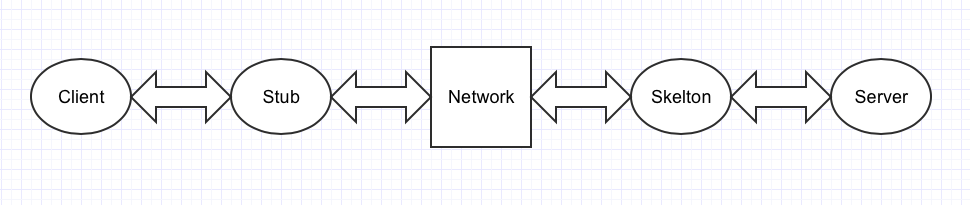
\includegraphics[scale=0.4]{javaRMI.png}
\end{center}

The diagram above illustrates the typical client-server communication with Java RMI. The first event that occurs is that the client is communicating with the stub. The stub acts as a gateway for client side object and all communication to the server side object are routed through it. After way to look at a stub is to think in terms of a proxy. The stub was a few responsibilities. These responsibilities include initiating the communication to the server skeleton using the network, translating calls from the caller object, passing arguments to the skeleton over the network, and informing the skeleton that the call is complete. After the stub has initiated this communication with the the skeleton over the network, the next thing to discuss is the purpose of the skeleton. The skeleton side acts as a gateway for server side objects and all incoming client requests are routed through this skeleton. This skeleton has a few responsibilities. These responsibilities include translating incoming data from the stub to the correct-up calls to server objects, passing argument to server objects, and passing values back to the client stub over the network. After this occurs, then the server will receive the message and the skeleton will have a response that is going to be sent the stub over the network an the client will receive the response from the server.
%----------------------------------------------------------------------------------------
%	SECTION 3
%----------------------------------------------------------------------------------------
\section{A document that summarizes two published papers that report on the use of Java RMI.}

The first paper that is going to be discussed demonstrates an approach by an Internet radio example \cite{Kapitza:2005:FRE:1101516.1101518}. The paper ``FORMI: An RMI Extension for Adaptive Applications" takes on the challenge to extend RMI so that it can cope with non-RPC based communication, fault tolerance, scalability, and quality-of-server in general \cite{Kapitza:2005:FRE:1101516.1101518}. In order to approach this challenge, the author of Rudiger Kapitza and Michael Kirstein present an RMI extension for supporting the very flexible fragmented-object model. The model of FORMI allows to build distributed objects with arbitrary internal communication protocols and interaction patterns \cite{Kapitza:2005:FRE:1101516.1101518}.

The second that was looked at focused on methodologies to enhance the streaming capabilities of the Java RMI \cite{Yang:2006:SSJ:1168054.1168063}. The paper ``Streaming Support for Java RMI in Distributed Environments" is able to enhance these video streaming capabilities in a couple of fashion. The first way is a support for Java RMI that includes a pushing mechanism which allows server to push data in a streaming fashion to the client side \cite{Yang:2006:SSJ:1168054.1168063}. The second way this paper enhanced the streaming capabilities of the Java RMI is by adding a aggregation mechanism which allows the client site to make a single remote invocation to gather data from multiple server that keep replicas of data streams and aggregate partial data into a complete data stream\cite{Yang:2006:SSJ:1168054.1168063}.

%----------------------------------------------------------------------------------------
%	SECTION 4
%----------------------------------------------------------------------------------------

\section{A paper that responds to the other questions that this assignment poses about Java RMI.}
\textbf{Question: Do you see any files that are specifically needed for a distributed system}

There is one specific that is need for this distributed system. This distributed system has a Simple.propreties file that specifies the port that the server is listening on and also specifies the server internet protocol (IP). 

\textbf{Question: At this point, you are ready to run the client and the server according to the commands that are provided in the documentation. What commands did you type? What output did they produce?}

In order to run the client and server correctly so that they communicate together, there were multiple commands that needed to be ran to achieve this. The follow list of commands are what was used to complete this laboratory assignment correctly.

\begin{itemize}
\item[ant compile]

This command compiles the program all together so you could get a bin directory.

\item[ant jar]

This command adds the jar files of the client and the server in the main directory.

\item[java -jar simple-server.jar]

This command starts the server

\item[java -jar simple-client.jar ping]

This command starts the client and sends the message ``Hello, world!" to the server

\end{itemize}
 
The next commands that were used were to test the commands of upload and download. 
 
\textbf{java -jar simple-client.jar upload ../../paper/a2-kapitza.pdf}

This command starts the client and uploads the following paper to the server

\textbf{java -jar simple-client jar download ../../paper/p42-yang.pdf}

This commands starts the client and download the following paper to the server. 


\textbf{Question: Can you determine the port used by the ``RMI registry" that this systems starts? Can you find the class that calls rebind? What is the purpose of this method?}

The port used by the ``RMI registry" is 1099. The class that class rebind is in the SimpleServer.java file. The purpose of this method is to replace the binding for the specified name in a specified registry opbject with the supplied remote reference so that remote object would be the SimpleImpl object.

%Questions To Answer:
%Do you see any files that are specifically needed for a distributed system
% After running "ant jar". What commnds did you type? What output did they produce?
%
% Can you determine the port used by the "RMI registry" that the system starts? Can you find the class that calls rebind? What is the prupose of this method?
%
%
%----------------------------------------------------------------------------------------
%	SECTION 5
%----------------------------------------------------------------------------------------
\section{A reflection on the challenges that you encountered when completing this assignment.}

There was one particular challenge that I had encountered when completing this assignment. This challenge included completing this laboratory assignment using Mac OS X. When I tried to run the commands presented in the assignment sheet of the laboratory assignment, it came to my attention that I did not have Apache ant installed on my MacBook Pro. To overcome this challenge, I had to use homebrew to install Apache Ant to ensure that I could compile and run this project. 

%----------------------------------------------------------------------------------------
%	BIBLIOGRAPHY
%----------------------------------------------------------------------------------------

\nocite{tanenbaum_steen_2007}
\nocite{Kapitza:2005:FRE:1101516.1101518}
\nocite{Yang:2006:SSJ:1168054.1168063}


\bibliographystyle{plain}
%\bibliographystyle{IEEEtran}
\bibliography{sample}

%----------------------------------------------------------------------------------------


\end{document}
